% tBPSguide.tex
% v2.1 released November 2014

\documentclass{tBPS2e}

\usepackage{epstopdf}% To incorporate .eps illustrations using PDFLaTeX, etc.
\usepackage{subfigure}% Support for small, `sub' figures and tables

\theoremstyle{plain}
\newtheorem{theorem}{Theorem}[section]
\newtheorem{lemma}[theorem]{Lemma}
\newtheorem{corollary}[theorem]{Corollary}
\newtheorem{proposition}[theorem]{Proposition}

\theoremstyle{definition}
\newtheorem{definition}{Definition}

\theoremstyle{remark}
\newtheorem{remark}{Remark}

\begin{document}

%\jvol{00} \jnum{00} \jyear{2014} \jmonth{November}

\articletype{GUIDE}

\title{\textit{Journal of Building Performance Simulation} \LaTeX\ guide for authors \break (Style 4 + Chicago author-date reference style)}

\author{
\name{A.N. Author\textsuperscript{a}$^{\ast}$\thanks{$^\ast$Corresponding author. Email: latex.helpdesk@tandf.co.uk}
and I.T. Consultant\textsuperscript{b}}
\affil{\textsuperscript{a}Taylor \& Francis, 4 Park Square, Milton Park, Abingdon, UK;
\textsuperscript{b}Institut f\"{u}r Informatik, Albert-Ludwigs-Universit\"{a}t, Freiburg, Germany}
\received{v2.1 released November 2014}
}

\maketitle

\begin{abstract}
This guide is for authors who are preparing papers for the Taylor \& Francis journal \textit{Journal of Building Performance Simulation}
(\textit{tBPS}) using the \LaTeX\ document preparation system and the class file \texttt{tBPS2e.cls}, which is available via the journal's home page on the Taylor \& Francis website.
\end{abstract}

\begin{keywords}
submission instructions; source file coding; environments; references citation; fonts; numbering
\bf{(Please provide three to six keywords taken from terms used in your manuscript)}
\end{keywords}


{\abstractfont\centerline{\bfseries Index to information contained in this guide}\vspace{12pt}
\hbox to \textwidth{\hsize\textwidth\vbox{\hsize19pc
\hspace*{-12pt} {1.}    Introduction\\
\hspace*{7pt} {1.1.}  The \textit{tBPS} document class\\
\hspace*{7pt} {1.2.}  Submission of \LaTeX\ articles\\
\hspace*{24pt}        to the journal\\
{2.}    Using the \textit{tBPS} class file\\
{3.}    Additional features\\
\hspace*{10pt}{3.1.}  Title, authors' names, abstract \\
\hspace*{24pt}        and keywords\\
\hspace*{10pt}{3.2.}  Additional footnotes to the title \\
\hspace*{24pt}        or authors' names\\
\hspace*{10pt}{3.3.}  Lists\\
{4.}    Some guidelines for using standard\\
\hspace*{6pt}         features\\
\hspace*{10pt}{4.1.}   Sections\\
\hspace*{10pt}{4.2.}   Illustrations (figures)\\
\hspace*{10pt}{4.3.}   Tables\\
\hspace*{10pt}{4.4.}   Landscape pages\\
\hspace*{10pt}{4.5.}   Theorem-like environments\\
\noindent \hspace*{7pt} {4.6.}   Typesetting mathematics\\
\hspace*{24pt} {4.6.1.}   Displayed mathematics\\
\hspace*{24pt} {4.6.2.}   Bold math italic symbols\\
\hspace*{24pt} {4.6.3.}   Bold Greek\\
\hspace*{24pt} {4.6.4.}   Upright Greek characters  \\
\hspace*{50pt}            and the upright partial \\
\hspace*{50pt}            derivative sign  \\}
\hspace{-24pt}\vbox{\noindent\hsize19pc
\hspace*{7pt} {4.7.}   Acknowledgements \\
\hspace*{7pt} {4.8.}   Funding \\
\hspace*{7pt} {4.9.}   Notes \\
\hspace*{7pt} {4.10.}   Supplemental material \\
\hspace*{7pt} {4.11.}   References \\
\hspace*{24pt} {4.11.1.}  References cited in the \\
\hspace*{54pt}            text \\
\hspace*{24pt} {4.11.2.}   The list of references\\
\hspace*{7pt} {4.12.}   Appendices \\
{5.}    Example of a section heading \\*
\hspace*{7pt}   including \textsc{small caps}, \textit{italic}, \\*
\hspace*{7pt}   and bold Greek such as ${\bm\kappa}$ \\
{6.}   {\em tBPS} journal style \\
\hspace*{10pt}{6.1.}   Hyphens, en rules, em rules \\ \hspace*{27pt}and minus signs\\
\hspace*{10pt}{6.2.}   References \\
\hspace*{10pt}{6.3.}   Maths fonts\\
\noindent   {7.}   Troubleshooting\\
{8.}   Fixes for coding problems\\
{9.}   Obtaining the tBPS2e class file\\
\hspace*{10pt}{9.1}  Via the Taylor \& Francis \\
\hspace*{24pt}       website \\
\hspace*{10pt}{9.2}  Via e-mail\\ }}}


\section{Introduction}

In order to assist authors in the process of preparing a manuscript for the \textit{Journal of Building Performance Simulation} (\textit{tBPS}), the journal's layout style has been implemented as a \LaTeXe\ class file based on the \texttt{article} document class. A \textsc{Bib}\TeX\ style file is also provided to assist with the formatting of your references in a style appropriate to that of the journal.

Commands that differ from or are provided in addition to the standard \LaTeXe\ interface are explained in this guide. The guide alone is not intended as a substitute for an appropriate \LaTeXe\ manual.

The \texttt{tBPSguide.tex} file can also be used as a template for composing an article for submission by cutting, pasting, inserting and
deleting text as appropriate, using the \LaTeX\ environments provided (e.g. \verb"\begin{equation}", \verb"\begin{enumerate}").

\textbf{Please note that the index following the abstract in this guide is provided for information only. An index is not required in submitted papers.}


\subsection{The \textit{tBPS} document class}\label{class}

The \textit{tBPS} class file preserves the standard \LaTeXe\ interface such that any document that can
be produced using \texttt{article.cls} can also be produced using the \textit{tBPS} document class.
However, the measure (the width of the text on a page) differs from the default for \texttt{article.cls}, therefore line breaks
will change and some long equations may need to be reformatted accordingly.

If your article is accepted for publication in the journal, it will be typeset in Monotype Times. As most authors do not own this font, the page make-up would inevitably alter with the change of font. Moreover, the class file produces single-column format, which is preferred for peer review and will be converted to two-column format by the typesetter. This also reduces formatting problems during preparation of papers by authors due to long lines and equations spanning more than one column. Line endings would change anyway during preparation of proofs from two-column format manuscripts because typesetters' character sets differ slightly in size from those available on most PCs and laptops. Please therefore ignore details such as slightly long lines of text, page stretching, figures or tables not appearing in exact synchronization with their citations in the text: these details will be dealt with by the typesetter. Similarly, it is unnecessary to spend time addressing warnings in the log file -- if your .tex file compiles to produce a PDF document that correctly shows how you wish your paper to appear, such warnings will not prevent your source files being imported into the typesetter's program.


\subsection{Submission of \LaTeX\ articles to the journal}\label{submission}

Manuscripts for possible publication in the journal should be submitted to the Editors for review as directed in the journal's Instructions for Authors, which may be found at \texttt{http://www.tandf.co.uk/journals/authors/tbpsauth.asp}.

Manuscripts created using \LaTeX\ should be converted to PDF format prior to submission. The \LaTeX\ source files and any graphics files will be required in addition to the final PDF version when final, revised versions of accepted manuscripts are submitted.

`Open-source' \LaTeXe\ should be used in preference to proprietary systems such as TCILaTeX or Scientific WorkPlace; similarly, class files such as REVTeX that produce a document in the style of a different publisher and journal should not be used for preference.

Please ensure that any author-defined macros are gathered together in the preamble of your .tex file, just before the
\verb"\begin{document}" command. Note that if serious problems are encountered with the coding of a paper (missing author-defined macros,
for example), it may prove necessary to divert the paper to conventional typesetting, i.e. it will be re-keyed.


\section{Using the \textit{tBPS} class file}

If the \texttt{tBPS2e} class file is not already in the appropriate system directory for \LaTeXe\ files, either
arrange for it to be put there, or copy it to your working folder. In order to use the \textit{tBPS} document class, replace the command
\verb"\documentclass{article}" at the beginning of your document with the command \verb"\documentclass{tBPS2e}".

The following document-class options should \emph{not} be used with the \textit{tBPS} class file:
\begin{itemize}
  \item \texttt{10pt}, \texttt{11pt}, \texttt{12pt} -- unavailable;
  \item \texttt{oneside}, \texttt{twoside} -- not necessary, oneside is the default;
  \item \texttt{leqno}, \texttt{titlepage} -- should not be used;
  \item \texttt{twocolumn} -- should not be used (see Section~\ref{class});
  \item \texttt{onecolumn} -- not necessary as it is the default style.
\end{itemize}
The \texttt{geometry} package and commands associated with it should also not be used to adjust the page dimensions.


\section{Additional features}

\subsection{Title, authors' names, abstract and keywords}

The title should be generated at the beginning of your article using the \verb"\maketitle" command.
In the final version, the author name(s) and affiliation(s) must be followed immediately by \verb"\maketitle" as shown below in order for them to be displayed in your PDF document.
To prepare an anonymous version for peer review, you can put the \verb"\maketitle" between the \verb"\title" and the \verb"\author" in order to conceal the authors' identities from the reviewers.
Next you should include an abstract, which should be enclosed within an \texttt{abstract} environment.
For example, the titles for this guide begin with the following source code:
\begin{verbatim}
\title{\textit{Journal of Building Performance Simulation} \LaTeX\
guide for authors (Style 4 + Chicago author-date reference style)}

\author{
\name{A.N. Author\textsuperscript{a}$^{\ast}$\thanks{$^\ast$Corresponding
author. Email: latex.helpdesk@tandf.co.uk}
and I.T. Consultant\textsuperscript{b}}
\affil{\textsuperscript{a}Taylor \& Francis, 4 Park Square, Milton Park,
Abingdon, UK; \textsuperscript{b}Institut f\"{u}r Informatik,
Albert-Ludwigs-Universit\"{a}t, Freiburg, Germany}
\received{v2.1 released November 2014} }

\maketitle

\begin{abstract}
This guide is for authors who are preparing papers for \textit{Journal
of Building Performance Simulation} (\textit{tBPS}) using the \LaTeX\
document preparation system and the class file \texttt{tBPS2e.cls},
which is available via the journal's home page on the Taylor \&
Francis website.
\end{abstract}
\end{verbatim}
A list of keywords should follow the abstract as required by the journal, enclosed within a \texttt{keywords} environment.


\subsection{Additional footnotes to the title or authors' names}

The \verb"\thanks" command may be used to produce additional footnotes to the title or authors' names if required.
Footnote symbols for this purpose should be used in the order:
$\dagger$ (coded as \verb"\dagger"), $\ddagger$ (\verb"\ddagger"), $\S$ (\verb"\S"), $\P$ (\verb"\P"), $\|$ (\verb"\|"),
$\dagger\dagger$ (\verb"\dagger\dagger"), $\ddagger\ddagger$ (\verb"\ddagger\ddagger"), $\S\S$ (\verb"\S\S"),\break
$\P\P$ (\verb"\P\P"), $\|\|$ (\verb"\|\|").
Note that any \verb"footnote"s to the \emph{main text} will automatically be assigned the superscript
 symbols 1, 2, 3, etc. by the class file.\footnote{If preferred, the \texttt{endnotes} package
 may be used to set the notes at the end of your text, before the bibliography.
 The symbols will be changed to match the style of the journal if necessary by the typesetter.}


\subsection{Lists}

The \textit{tBPS} class file provides numbered and unnumbered lists using the \texttt{enumerate} environment and bulleted
lists using the \texttt{itemize} environment.

The enumerated list will number each list item with arabic numerals by default. For example,
\begin{enumerate}
  \item first item
  \item second item
  \item third item
\end{enumerate}
was produced by
\begin{verbatim}
\begin{enumerate}
  \item first item
  \item second item
  \item third item
\end{enumerate}
\end{verbatim}
Alternative numbering styles can be achieved by inserting an optional argument in square brackets to each \verb"\item", e.g. \verb"\item[(i)] first item" to create a list numbered with roman numerals.

Unnumbered lists can also be produced using the \texttt{enumerate} environment. For example,
\begin{enumerate}
  \item[] First unnumbered item
  \item[] Second unnumbered item
  \item[] Third unnumbered item
\end{enumerate}
was produced by
\begin{verbatim}
\begin{enumerate}
  \item[] First unnumbered item
  \item[] Second unnumbered item
  \item[] Third unnumbered item
\end{enumerate}
\end{verbatim}

Bulleted lists are provided using the \texttt{itemize} environment. For example,
\begin{itemize}
  \item First bulleted item
  \item Second bulleted item
  \item Third bulleted item
\end{itemize}
was produced by
\begin{verbatim}
\begin{itemize}
  \item First bulleted item
  \item Second bulleted item
  \item Third bulleted item
\end{itemize}
\end{verbatim}


\section{Some guidelines for using standard features}

The following notes are intended to help you achieve the best effects with the \texttt{tBPS2e} class file.


\subsection{Sections}

\LaTeXe\ provides five levels of section heading, all of which are defined in the \texttt{tBPS2e} class file:
\begin{enumerate}
  \item[(A)] \verb"\section"
  \item[(B)] \verb"\subsection"
  \item[(C)] \verb"\subsubsection"
  \item[(D)] \verb"\paragraph"
  \item[(E)] \verb"\subparagraph"
\end{enumerate}
Numbering is automatically generated for section, subsection, subsubsection and paragraph headings. If you need
additional text styles in the headings, see the examples given in Section~\ref{headings}.


\subsection{Illustrations (figures)}

See `Instructions for Authors' in the journal's home page on the Taylor \& Francis website for how to submit artwork (note that requests to supply figures and tables separately from text are for the benefit of authors using Microsoft Word; authors using \LaTeX\ may incorporate these at the appropriate locations). The source files of any illustrations will be required when the final, revised version is submitted. Authors should ensure that their figures are suitable (in terms of lettering size, etc.) for the reductions they intend.

The \textit{tBPS} class file will cope with most positioning of your illustrations and you should not normally need to use the optional placement specifiers of the \texttt{figure} environment.
Figure captions should appear below the figure itself, therefore the \verb"\caption" command should appear after the figure.
For example, Figure~\ref{sample-figure} with caption and sub-captions is produced using the following commands:
\begin{verbatim}
\begin{figure}
\begin{center}
\begin{minipage}{130mm}
\subfigure[An example of an individual figure sub-caption.]{
\resizebox*{6cm}{!}{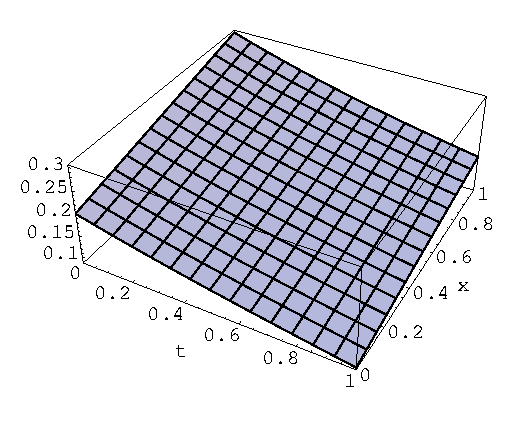
\includegraphics{senu_gr1.eps}}}\hspace{6pt}
\subfigure[A slightly shorter sub-caption.]{
\resizebox*{6cm}{!}{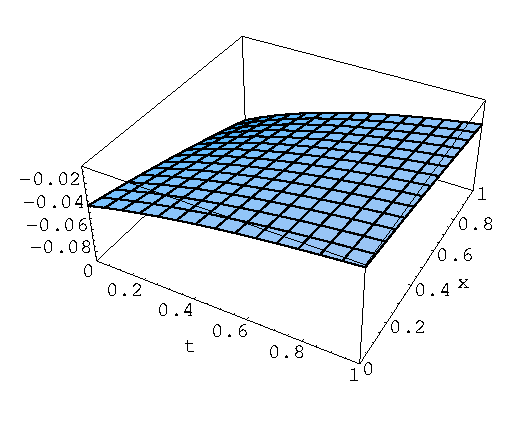
\includegraphics{senu_gr2.eps}}}
\caption{Example of a two-part figure with individual sub-captions
 showing that captions are flush left and justified if greater
 than one line.} \label{sample-figure}
\end{minipage}
\end{center}
\end{figure}
\end{verbatim}

\begin{figure}
\begin{center}
\begin{minipage}{130mm}
\subfigure[An example of an individual figure sub-caption.]{
\resizebox*{6cm}{!}{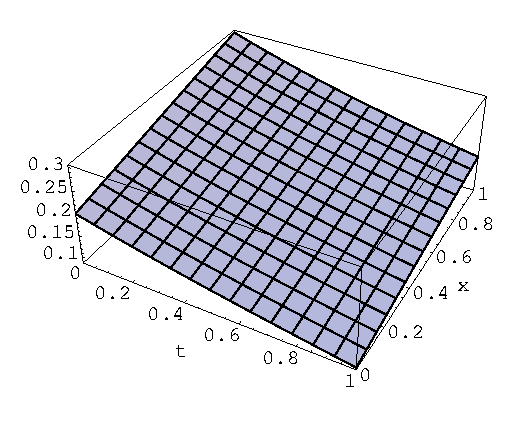
\includegraphics{senu_gr1.eps}}}\hspace{6pt}
\subfigure[A slightly shorter sub-caption.]{
\resizebox*{6cm}{!}{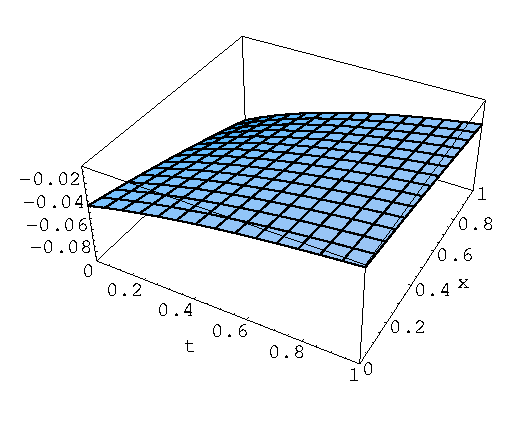
\includegraphics{senu_gr2.eps}}}
\caption{Example of a two-part figure with individual sub-captions
 showing that captions are flush left and justified if greater
 than one line.} \label{sample-figure}
\end{minipage}
\end{center}
\end{figure}

The \verb"\subfigure{}" and \verb"\includegraphics{}" commands require subfigure.sty and graphicx.sty.
The former is called in the preamble of the \texttt{tBPSguide.tex} file (in order to allow your choice of an alternative package if preferred)
and the latter by the \texttt{tBPS2e} class file; both are included with the \LaTeX\ style guide package for this journal for convenience.
Please supply any additional figure macros you use with your article in the preamble of your .tex file before \verb"\begin{document}".

To ensure that figures are correctly numbered automatically, the \verb"\label{}" command should be inserted just
after the \verb"\caption{}" command, or in its argument.

The \texttt{epstopdf} package can be used to incorporate Encapsulated PostScript (.eps) illustrations when using PDF\LaTeX, etc.
Please provide the original .eps source files rather than the generated PDF images of those illustrations for production purposes.


\subsection{Tables}

The \textit{tBPS} class file will cope with most positioning of your tables and you should not normally need to use the optional
placement specifiers of the \texttt{table} environment.

The \texttt{tabular} environment can be used as illustrated here to produce tables with appropriately spaced single thick and thin
horizontal rules, which are allowed, if desired. Thick rules should be used at the head and foot only, and thin rules elsewhere as appropriate.
Commands to redefine quantities such as \verb"\arraystretch" should be omitted.

The table caption appears above the body of the table in \textit{tBPS} style, therefore the \verb"\tbl" command should be used before the body of the table.
For example, Table~\ref{sample-table} is produced using the following commands. Note that \verb"\rm" will produce a roman character in math mode.
There are also \verb"\bf" and \verb"\it", which produce bold face and text italic in math mode.

\begin{table}
\tbl{Example of a table showing that its caption is as wide as the
  table itself and justified.}
{\begin{tabular}[l]{@{}lcccccc}\toprule
  Class$^{\rm a}$ & $\gamma _1$ & $\gamma _2$$^{\rm b}$
         & $\langle \gamma \rangle$ & $G$ & $|{\bm f}|$ & $\theta _{c}$ \\
\colrule
  BL Lacs & 5 & 36 & 7 & $-4.0$ & $1.0\times 10^{-2}$ & 10$^\circ$ \\
  FSRQs & 5 & 40 & 11 & $-2.3$ & $0.5\times 10^{-2}$ & 14$^\circ$ \\
\botrule
\end{tabular}}
\tabnote{$^{\rm a}$This footnote shows what footnote symbols to use.}
\tabnote{$^{\rm b}$This footnote shows the text turning over when a long footnote is added.}
\label{sample-table}
\end{table}

\begin{verbatim}
\begin{table}
\tbl{Example of a table showing that its caption is as wide as the
 table itself and justified.}
{\begin{tabular}[l]{@{}lcccccc}\toprule
   Class$^{\rm a}$ & $\gamma _1$ & $\gamma _2$$^{\rm b}$
         & $\langle \gamma \rangle$ & $G$ & $|{\bm f}|$ & $\theta _{c}$ \\
\colrule
   BL Lacs & 5 & 36 & 7 & $-4.0$ & $1.0\times 10^{-2}$ & 10$^\circ$ \\
   FSRQs & 5 & 40 & 11 & $-2.3$ & $0.5\times 10^{-2}$ & 14$^\circ$ \\
\botrule
\end{tabular}}
\tabnote{$^{\rm a}$This footnote shows what footnote symbols to use.}
\tabnote{$^{\rm b}$This footnote shows the text turning over when
 a long footnote is added.}
\label{sample-table}
\end{table}
\end{verbatim}

To ensure that tables are correctly numbered automatically, the \verb"\label{}" command should be inserted just before \verb"\end{table}".
Tables produced using the \texttt{booktabs} package of macros for typesetting tables are also compatible with the \textit{tBPS} class file.


\subsection{Landscape pages}\label{landscape}

If a table or illustration is too wide to fit the measure it will need to be turned, along with its caption, through 90$^{\circ}$ anticlockwise.
Landscape illustrations and/or tables can be produced using the \verb"rotating" package, which is called by the \textit{tBPS} class file.
The following commands (for example) can be used to produce such pages.
\begin{verbatim}
\setcounter{figure}{0}
\begin{sidewaysfigure}
\centerline{\epsfbox{figname.eps}}
\caption{Example landscape figure caption.}
\label{landfig}
\end{sidewaysfigure}
\end{verbatim}

\begin{verbatim}
\setcounter{table}{0}
\begin{sidewaystable}
 \tbl{Example landscape table caption.}
  {\begin{tabular}{@{}llllcll}
    .
    .
    .
  \end{tabular}}\label{landtab}
\end{sidewaystable}
\end{verbatim}
Before any such float environment, use the \verb"\setcounter" command as above to fix the numbering of the caption. Subsequent captions will then be automatically renumbered accordingly.

The \verb"\epsfbox{}" command requires epsfig.sty, which is called by the \texttt{tBPS2e} class file and included with the \LaTeX\ style guide package for this journal for convenience.


\subsection{Theorem-like environments}

A predefined \verb"proof" environment is provided by the \texttt{amsthm} package (which is called by the class file), as follows:

\begin{proof}
More recent algorithms for solving the semidefinite programming
relaxation are particularly efficient, because they explore the
structure of the MAX-CUT problem.
\end{proof}
\noindent This was produced by simply typing:
\begin{verbatim}
\begin{proof}
More recent algorithms for solving the semidefinite programming
relaxation are particularly efficient, because they explore the
structure of the MAX-CUT problem.
\end{proof}
\end{verbatim}
Other theorem-like environments (theorem, lemma, corollary, etc.) need to be defined as required, e.g. using \verb"\newtheorem{theorem}{Theorem}[section]"
in the preamble of your .tex file before \verb"\begin{document}". Theorem-like structures in \textit{tBPS} are generally numbered as per the following examples:

\begin{theorem}
More recent algorithms for solving the semidefinite programming
relaxation are particularly efficient, because they explore the
structure of the MAX-CUT problem.
\end{theorem}
\begin{lemma}
More recent algorithms for solving the semidefinite programming
relaxation are particularly efficient, because they explore the
structure of the MAX-CUT problem.
\end{lemma}
\begin{corollary}
More recent algorithms for solving the semidefinite programming
relaxation are particularly efficient, because they explore the
structure of the MAX-CUT problem.
\end{corollary}
\begin{proposition}
More recent algorithms for solving the semidefinite programming
relaxation are particularly efficient, because they explore the
structure of the MAX-CUT problem.
\end{proposition}
\begin{definition}
More recent algorithms for solving the semidefinite programming
relaxation are particularly efficient, because they explore the
structure of the MAX-CUT problem.
\end{definition}
\begin{remark}
More recent algorithms for solving the semidefinite programming
relaxation are particularly efficient, because they explore the
structure of the MAX-CUT problem.
\end{remark}

\noindent These were defined as shown in detail in the preamble of the \texttt{tBPSguide}.tex file, and produced by typing, for example:
\begin{verbatim}
\begin{theorem}
More recent algorithms for solving the semidefinite programming
relaxation are particularly efficient, because they explore the
structure of the MAX-CUT problem.
\end{theorem}
\end{verbatim}
The format of the text in these environments may be changed if necessary to match the style of the journal by the typesetter during preparation of your proofs.


\subsection{Typesetting mathematics}\label{TMth}

\subsubsection{Displayed mathematics}

The \textit{tBPS} class file will set displayed mathematics centred on the measure without equation numbers if the \LaTeX\ standard commands open (\verb"\[") and close (\verb"\]") square brackets are used as
delimiters. The equation
\[
  \sum_{i=1}^p \lambda_i = {\rm trace}({\textrm{\bf S}})\qquad
  i\in {\mathbb R}
\]
\normalfont was typeset using the commands
\begin{verbatim}
\[
  \sum_{i=1}^p \lambda_i = {\rm trace}({\textrm{\bf S}})\qquad
  i\in {\mathbb R}
\]
\end{verbatim}

For those of your equations that you wish to be automatically numbered sequentially throughout the text, use the \texttt{equation} environment, e.g.
\begin{equation}
  \sum_{i=1}^p \lambda_i = {\rm trace}({\textrm{\bf S}})\qquad
  i\in {\mathbb R}
\end{equation}
was typeset using the commands
\begin{verbatim}
\begin{equation}
  \sum_{i=1}^p \lambda_i = {\rm trace}({\textrm{\bf S}})quad
  i\in {\mathbb R}
\end{equation}
\end{verbatim}

Part numbers for sets of equations may be generated using the \texttt{subequations} environment, e.g.
\begin{subequations} \label{subeqnexample}
\begin{equation}
        \varepsilon \rho w_{tt}(s,t)
        =
        N[w_{s}(s,t),w_{st}(s,t)]_{s},
        \label{subeqnpart}
\end{equation}
\begin{equation}
        w_{tt}(1,t)+N[w_{s}(1,t),w_{st}(1,t)] = 0,
\end{equation}
\end{subequations}
which was generated using the commands
\begin{verbatim}
\begin{subequations} \label{subeqnexample}
\begin{equation}
        \varepsilon \rho w_{tt}(s,t)
        =
        N[w_{s}(s,t),w_{st}(s,t)]_{s},
        \label{subeqnpart}
\end{equation}
\begin{equation}
        w_{tt}(1,t)+N[w_{s}(1,t),w_{st}(1,t)] = 0,
\end{equation}
\end{subequations}
\end{verbatim}
This is made possible by the \texttt{subeqn} package, which is called by the class file.
If you put the \verb"\label{}" just after the \verb"\begin{subequations}" line, references will be to the
collection of equations, `(\ref{subeqnexample})' in the example above.
Or, like the example code above, you can reference each equation individually -- e.g. `(\ref{subeqnpart})'.

Displayed mathematics should be given end-of-line punctuation appropriate to the running text sentence of which it forms a part, if required.

\subsubsection{Bold math italic symbols}

To get bold math italic you can use \verb"\bm", which works for all sizes, e.g.
\begin{verbatim}
\sffamily
\begin{equation}
   {\rm d}({\bm s_{t_{\bm u}}) = \langle{\bm\alpha({\sf{\textbf L}})}
   [RM({\bm X}_y + {\bm s}_t) - RM({\bm x}_y)]^2 \rangle
\end{equation}
\normalfont
\end{verbatim}
produces\sffamily
\begin{equation}
   {\rm d}({\bm s_{t_{\bm u}}}) = \langle {\bm\alpha({\sf{\textbf L}})}[RM({\bm X}_y
   + {\bm s}_t) - RM({\bm x}_y)]^2 \rangle
\end{equation}\normalfont
Note that subscript, superscript, subscript to subscript, etc.
sizes will take care of themselves and are italic, not bold,
unless coded individually. \verb"\bm" produces the same effect as
\verb"\boldmath". \verb"\sffamily"...\verb"\normalfont" allows
upright sans serif fonts to be created in math mode by using the
control sequence `\verb"\sf"'.

\subsubsection{Bold Greek}\label{boldgreek}

Bold lowercase as well as uppercase Greek characters can be
obtained by \verb"{\bm \gamma}", which gives ${\bm \gamma}$, and
\verb"{\bm \Gamma}", which gives ${\bm \Gamma}$.

\subsubsection{Upright lowercase Greek characters and the upright partial derivative sign}\label{upgreek}

Upright lowercase Greek characters can be obtained with the \textit{tBPS} class file by inserting the letter `u' in the control
code for the character, e.g. \verb"\umu" and \verb"\upi" produce $\umu$ (used, for example, in the symbol for the
unit microns -- $\umu{\rm m}$) and $\upi$ (the ratio of the circumference to the diameter of a circle). Similarly,
the control code for the upright partial derivative $\upartial$ is \verb"\upartial".


\subsection{Acknowledgements}

An unnumbered section, e.g. \verb"\section*{Acknowledgement(s)}", should be used for thanks, etc.
and placed \emph{in the non-anonymous version} before any Notes or References sections.


\subsection{Funding}

An unnumbered section, e.g. \verb"\section*{Funding}", should be used for grant details, etc.
and placed \emph{in the non-anonymous version} before any Notes or References sections.


\subsection{Notes}

An unnumbered Notes section may be placed before the References section. If using the \verb"endnotes" package, use the command \verb"\theendnotes" to create this section.


\subsection{Supplemental material}

Supplemental material should be referenced within your article where appropriate. An unnumbered section, e.g. \verb"\section*{Supplemental material}", detailing the supplemental material available should be placed immediately before the list of references, and should include a brief description of each supplemental file.


\subsection{References}\label{refs}

\subsubsection{References cited in the text}

References should be cited in the text in `Chicago author-date' style, separated by semi-colons, e.g. (Green 2002; Harlow 1983; Wegener and Petty 1994) or `...~see Smith (1985,~75)'. If there are two authors with the same surname, use the first initials with the surnames, e.g. (E.~Johnson 2001; L.~Johnson 1998). If there are three authors, list them all in every citation, e.g. (Kernis, Cornell, and Harlow 1993). For more than three authors, cite the first author's name followed by et al. For two or more sources by the same author(s) in the same year, use lower-case letters (a, b, c,...) with the year to order the entries in the Reference list and use these letters with the year in the in-text citations, e.g. (Green 1981a,b). Further details on this reference style can be found in the journal's Instructions for Authors.

Each bibliographical entry has a key, which is assigned by the author and used to refer to that entry in the text. In this document, the key \verb"ev94" in the citation form \verb"\citep{ev94}" produces `\citep{ev94}', and the keys in the citation \verb"\citep{Eri1984,GloRib51,PeaEtAl76}" produce `\citep{Eri1984,GloRib51,PeaEtAl76}'. The appropriate citation style for different situations can be obtained, for example, by \verb"\citet{hk97}" for `\citet{hk97}', \verb"\citet{Bar91,Mil93,Maz91}" for `\citet{Bar91,Mil93,Maz91}', or \verb"\citealt{Holl04}" for `\citealt{Holl04}'. Optional notes may be included at the beginning and end of a citation by the use of square brackets, e.g. \verb"\citep[see][123]{Agu95}" produces `\citep[see][123]{Agu95}'. Citation of the year alone may be produced by \verb"\citeyear{cwm73}", i.e. `\citeyear{cwm73}', or \verb"\citeyearpar{glov86}", i.e. `\citeyearpar{glov86}'.

\subsubsection{The list of references}

References should be listed at the end of the main text in alphabetical order, then chronologically (earliest first), with full page ranges (where appropriate) and issue numbers (for journals paginated by issue). If a reference has more than ten named authors, list only the first seven, followed by `et al.'. The following list shows some sample references prepared in the style of the journal.

\begin{thebibliography}{99}

\bibitem[Agutter(1995)]{Agu95}
Agutter, A.~J. 1995. ``The Linguistic Significance of Current {B}ritish
 Slang.'' Unpublished doctoral dissertation, Edinburgh University, UK.

\bibitem[Barlow(1991)]{Bar91}
Barlow, D.~H. 1991. ``Diagnoses, Dimensions, and {DSM-IV} [Special issue].''
 \emph{Journal of Abnormal Psychology} 100 (3).

\bibitem[Ericsson and Simon(1984)]{Eri1984}
Ericsson, K.~Anders, and Herbert~A. Simon. 1984. \emph{Protocol Analysis:
 Verbal Reports as Data}. Cambridge, MA: MIT Press.

\bibitem[Evans(1994)]{ev94}
Evans, W.~A. 1994. ``Approaches to Intelligent Information Retrieval.''
 \emph{Information Processing and Management} 7 (2): 147--168.

\bibitem[Glover(1986)]{glov86}
Glover, Fred. 1986. ``Hilbert Modular Forms and the {G}alois Representations
 Associated to {H}ilbert--{B}lumenthal Abelian Varieties.'' Ph.D. thesis,
 Harvard University, Cambridge, MA.

\bibitem[Glover, Smith, and Ribeiro(1951)]{GloRib51}
Glover, Fred, Raymond Smith, and C.~C. Ribeiro, eds. 1951. \emph{Lessons of the {B}ritish War
 Economy}. vol.~5. 2nd ed. Westport, CT: Greenwood Press.

\bibitem[Holland(2004)]{Holl04}
Holland, M. 2004. ``Guide to Citing Internet Sources.'' Accessed~November 4,
 2012.
 http://www.bournemouth.ac.uk/library/using/guide\_to\_citing\_internet\_sourc.html.

\bibitem[Kern(1997)]{hk97}
Kern, Hudson. 1997. ``The Resurgent {J}apanese Economy and a {J}apan--{U}nited
 {S}tates Free Trade Agreement.'' In \emph{4th International Conference on the
 Restructuring of the Economic and Political System in {J}apan and {E}urope},
 edited by C.~Lambert and G.~Holst. Milan, Italy, 21--25 May 1996. 147--156.
 Singapore: World Scientific.

\bibitem[Mazzeo(1991)]{Maz91}
Mazzeo, J. 1991. \emph{Comparability of Computer and Paper-and-Pencil Scores}
 (College Board Rep. No. 91). Princeton, NJ: Educational Testing Service.

\bibitem[Miller(1993)]{Mil93}
Miller, M.~E. 1993. \emph{The Interactive Tester (Version 4.0) [Computer
 software]}. Westminster, CA: Psytek Services.

\bibitem[Misner(1973)]{cwm73}
Misner, Charles~W. 1973. ``Efficient Algorithms for Layer Assignment
 Problems.'' In \emph{Gravitation in a Collapsing {U}niverse}, Vol.~5 of
 \emph{Einstein's Legacy}, edited by Ignatius Gottlob. 2nd ed. 63--83. San
 Francisco, CA: Freeman.

\bibitem[Pierce et~al.(1976)]{PeaEtAl76}
Pierce, Ian~F., Fred Glover, A.~T. Ogilvy, and A.~R.~S. Clements. 1976.
 ``A Model of Output, Employment, Wages and Prices in the {UK}.'' In
 \emph{Computing Tools for Modeling, Optimization and Simulation: Interfaces
 in Computer Science and Operations Research}, edited by Manuel Laguna and
 Jos\'{e}~Luis Gonz\'{a}les-Velarde. 2nd ed. 1--24. Boston, MA:
 Cambridge University Press.

\end{thebibliography}
\bigskip
\noindent This was produced by typing:
\begin{verbatim}
\begin{thebibliography}{99}

\bibitem[Agutter(1995)]{Agu95}
Agutter, A.~J. 1995. ``The Linguistic Significance of Current {B}ritish 
 Slang.'' Unpublished doctoral dissertation, Edinburgh University, UK.

\bibitem[Barlow(1991)]{Bar91}
Barlow, D.~H. 1991. ``Diagnoses, Dimensions, and {DSM-IV} [Special
 issue].'' \emph{Journal of Abnormal Psychology} 100 (3).

\bibitem[Ericsson and Simon(1984)]{Eri1984}
Ericsson, K.~Anders, and Herbert~A. Simon. 1984. \emph{Protocol
 Analysis: Verbal Reports as Data}. Cambridge, MA: MIT Press.

\bibitem[Evans(1994)]{ev94}
Evans, W.~A. 1994. ``Approaches to Intelligent Information Retrieval.''
 \emph{Information Processing and Management} 7 (2): 147--168.

\bibitem[Glover(1986)]{glov86}
Glover, Fred. 1986. \emph{Hilbert Modular Forms and the {G}alois 
 Representations Associated to {H}ilbert--{B}lumenthal Abelian 
 Varieties}. Ph.D. thesis, Harvard University, Cambridge, MA.

\bibitem[Glover, Smith, and Ribeiro(1951)]{GloRib51}
Glover, Fred, Raymond Smith, and C.~C. Ribeiro, eds. 1951.
 \emph{Lessons of the {B}ritish War Economy}. vol.~5. 2nd ed.
 Westport, CT: Greenwood Press.

\bibitem[Holland(2004)]{Holl04}
Holland, M. 2004. ``Guide to Citing Internet Sources.'' Accessed
 November 4, 2012.
 http://www.bournemouth.ac.uk/library/using/guide\_to\_citing\_internet\_sourc.html.

\bibitem[Kern(1997)]{hk97}
Kern, Hudson. 1997. ``The Resurgent {J}apanese Economy and a
 {J}apan--{U}nited {S}tates Free Trade Agreement.'' In \emph{4th
 International Conference on the Restructuring of the Economic and
 Political System in {J}apan and {E}urope}, edited by C.~Lambert
 and G.~Holst. Milan, Italy, 21--25 May 1996. 147--156. Singapore:
 World Scientific.

\bibitem[Mazzeo(1991)]{Maz91}
Mazzeo, J. 1991. \emph{Comparability of Computer and Paper-and-Pencil
 Scores} (College Board Rep. No. 91). Princeton, NJ: Educational
 Testing Service.

\bibitem[Miller(1993)]{Mil93}
Miller, M.~E. 1993. \emph{The Interactive Tester (Version 4.0)
 [Computer software]}. Westminster, CA: Psytek Services.

\bibitem[Misner(1973)]{cwm73}
Misner, Charles~W. 1973. ``Efficient Algorithms for Layer Assignment
 Problems.'' In \emph{Gravitation in a Collapsing {U}niverse},
 Vol.~5 of \emph{Einstein's Legacy}, edited by Ignatius Gottlob.
 2nd ed. 63--83. San Francisco, CA: Freeman.

\bibitem[Pierce et~al.(1976)]{PeaEtAl76}
Pierce, Ian~F., Fred Glover, A.~T. Ogilvy, and A.~R.~S. Clements. 1976.
 ``A Model of Output, Employment, Wages and Prices in the {UK}.''
 In \emph{Computing Tools for Modeling, Optimization and Simulation:
 Interfaces in Computer Science and Operations Research}, edited
 by Manuel Laguna and Jos\'{e}~Luis Gonz\'{a}les-Velarde. 2nd ed.
 1--24. Boston, MA: Cambridge University Press.

\end{thebibliography}
\end{verbatim}
\medskip
\noindent Each entry takes the form:
\begin{verbatim}
\bibitem[authors' names(date of publication)]{key}
Bibliography entry
\end{verbatim}
\noindent where `\texttt{authors' names}' is the list of names to appear where the \verb"bibitem" is cited in the text, and `\texttt{key}' is the tag that is to be used as an argument for the \verb"\cite{}" commands in the text of the article. \texttt{Bibliography entry} should be the material that is to appear in the list of references, suitably formatted.

Instead of typing the bibliography by hand, you may prefer to create the list of references using a \textsc{Bib}\TeX\ database. Include the lines
\begin{verbatim}
\bibliographystyle{tBPS}
\bibliography{tBPSguide}
\end{verbatim}
where the list of references should appear, where \texttt{tBPS.bst} is the name of the \textsc{Bib}\TeX\ style file for this journal and \texttt{tBPSguide.bib} is the database of bibliographic details for the references section included with the \textit{tBPS} \LaTeX\ style guide package (to be replaced with the name of your own \textsc{Bib}\TeX\ database). The \LaTeX\ source file of your paper will extract from your .bib file only those references that are cited in that paper and list them in the References section of it.

Please include a copy of your .bib file and/or the final generated .bbl file among your source files if your .tex file does not contain a reference list in a \texttt{thebibliography} environment.


\subsection{Appendices}\label{appendices}

Any appendices should be placed after the list of references, beginning with the
command \verb"\appendices" followed by the command \verb"\section" for each appendix title, e.g.
\begin{verbatim}
\appendices
\section{This is the title of the first appendix}
\section{This is the title of the second appendix}
\end{verbatim}
\noindent produces:\medskip

\noindent\textbf{Appendix A. This is the title of the first appendix}\vspace{12pt}

\noindent\textbf{Appendix B. This is the title of the second appendix}

\medskip
\noindent Subsections, equations, figures, tables, etc. within appendices will then be automatically numbered as appropriate.


\section{Example of a section heading including {\fontencoding{T1}\scshape{small caps}},
   {\bi italic}, and bold Greek such as ${\bm\kappa}$}\label{headings}

The following code shows how to achieve this section heading:
\begin{verbatim}
\section{Example of a section heading including
 {\fontencoding{T1}\scshape{small caps}}, {\bi italic},
 and bold Greek such as ${\bm\kappa}$}\label{headings}
\end{verbatim}


\section{\textit{tBPS} journal style}

The notes given here relate to common style errors found in manuscripts, but are \emph{not} intended to be exhaustive.


\subsection{Hyphens, en rules, em rules and minus signs}\label{dashes}

\begin{enumerate}
\item[(i)] Hyphens (one dash in \TeX/\LaTeX). \textit{tBPS} uses hyphens for compound adjectives (e.g.\ low-density gas, least-squares fit,
two-component model) but not for complex units or ranges, which could become cumbersome (e.g.\ 15~km~s$^{-1}$
feature, 100--200~$\umu$m observations).

\item[(ii)] en rules (two dashes in \TeX/\LaTeX). These are used (a) to denote a range (e.g.\ 1.6--2.2~$\umu$m);
(b) to denote the joining of two words of equal standing (e.g.\ Kolmogorov--Smirnov  test, Herbig--Haro object);
(c) with spaces, as an alternative to parentheses (e.g.\ `the results -- assuming no temperature gradient -- are indicative of \ldots').

\item[(iii)] The em rule (three dashes in \TeX/\LaTeX) has no specified use in \textit{tBPS}.

\item[(iv)] The minus sign is produced automatically in math mode by the use of a single dash, e.g.
\begin{equation}
y_{i} \in \{-1, 1 \} \quad \forall i \in V,
\end{equation}
\noindent where $|-V|=A^2+B^2.$\medskip

\noindent is produced by
\begin{verbatim}
\begin{equation}
y_{i} \in \{-1, 1 \} \quad \forall i \in V,
\end{equation}
\noindent where $|-V|=A^2+B^2.$
\end{verbatim}

\end{enumerate}


\subsection{References}

It is important to use the correct reference style, details of which can be found in Section~\ref{refs}.


\subsection{Maths fonts}

Scalar variables should be mediumface italic (e.g.\ $s$ for speed); vectors 
should be bold italic (e.g.\ $\bm v$ for velocity); matrices should be bold 
roman (upright) (e.g.\ $\bf A$), and tensors should be bold upright sans serif
(e.g.\ {\sffamily{\textbf L}}). Differential d, partial differential $\upartial$, 
complex i, exponential e, superscript T for `transpose', sin, cos, tan, log,
etc., should all be roman. Openface, or `blackboard', fonts can be used, for 
example, for the integers $\mathbb Z$ and the reals $\mathbb R$. 
Sub/superscripts that are physical variables should be italic, while those 
that are labels should be roman (e.g.\ $C_p$, $T_{\rm eff}$).


\section{Troubleshooting}

Authors may from time to time encounter problems with the preparation of a
paper in \LaTeX. The appropriate action to take will depend on the nature of
the problem -- the following is intended as a guide.

\begin{enumerate}
\item[(i)] If the problem is with \LaTeX\ itself, rather than with the
actual macros, please refer to an appropriate handbook for
initial advice. If the solution cannot be found, or if you
suspect that the problem lies with the macros, then please contact
Taylor \& Francis for assistance (\texttt{latex.helpdesk@tandf.co.uk}).

\item[(ii)] Problems with page make-up (e.g.\ large spaces between paragraphs,
above headings, or below figures; figures/tables appearing out of order):
please do not attempt to remedy these using `hard' page make-up
commands -- the typesetter will deal with such problems. (You may, if you
wish, draw attention to particular problems when submitting the final version
of your paper.)

\item[(iii)] If a required font is not available at your site, allow \TeX\
to substitute the font and specify which font you require in a
covering letter accompanying your file(s).
\end{enumerate}


\section{Fixes for coding problems}

This guide has been designed to minimize the need for user-defined macros to create special symbols. Authors
are urged, wherever possible, to use the following coding rather than to create their own. This will minimize
the danger of author-defined macros being accidentally `overridden' when the paper is typeset (see
Section~\ref{TMth}, `Typesetting mathematics'). In cases where it is essential to create your own macros,
these should be displayed in the preamble of the source file before \verb"\begin{document}".
%
\begin{enumerate}
\item[(i)] Fonts in section headings and paper titles. The following are examples
of styles that sometimes prove difficult to code.

\subsection*{Paper titles:}

\hsize380pt\bf{\noindent Generalized Flory theory at ${\bm\delta >
{\bf 50}^\circ}$}\\

    \noindent\normalfont is produced by
\begin{verbatim}
\title{Generalized Flory theory at
        ${\bm\delta > {\bfseries 50}^\circ}$}
\end{verbatim}
\bigskip

{\bf{\noindent Ion--ion correlations in H\,{\sc ii} regions}}\\

\noindent\normalfont is produced by
\begin{verbatim}
\title{Ion--ion correlations in H\,{\sc ii} regions}
\end{verbatim}


\stepcounter{enumi}

\item[(ii)] en rules, em rules, hyphens and minus signs (see Section~\ref{dashes} for
correct usage). To create the correct symbols in the sentence
\begin{quote}
The high-resolution observations were made along a line at an
angle of $-15^\circ$ (East from North) from the axis of the
jet -- which runs North--South
\end{quote}
you would use the following code:
\begin{verbatim}
The high-resolution observations were made along a line at an
angle of $-15^\circ$ (East from North) from the axis of the
jet -- which runs North--South
\end{verbatim}

\item[(iii)] Fonts in superscripts and subscripts. Subscripts and superscripts will automatically come out in the correct font
and size in a math environment (e.g.\ enclosed by `\verb"$"'
delimiters in running text or within \verb"\[...\]" or the
`\texttt{equation}' environment for displayed equations). You can create
the output ${\bm k_x}$ by typing \verb"${\bm k_x}$". If the
subscripts or superscripts need to be other than italic, they
should be coded individually -- see (vi) below.

\item[(iv)] Calligraphic letters ($\mathcal{UPPER\ CASE\ ONLY}$).
Normal calligraphic can be produced with \verb"\mathcal" as usual (in
math mode).

\item[(v)] Automatic scaling of brackets. The codes \verb"\left" and
\verb"\right" should  be used to scale brackets automatically to
fit the equation being set. For example, to get
\[
   v = x \left( \frac{N+2}{N} \right)
\]
use the code
\begin{verbatim}
\[
   v = x \left( \frac{N+2}{N} \right)
\]
\end{verbatim}

\item[(vi)] Roman font in equations. It is often necessary to make some
symbols roman in an equation (e.g.\ units, non-variable
subscripts). For example, to get
\[
   \sigma \simeq (r/13~h^{-1}~{\rm Mpc})^{-0.9},
   \qquad \omega = \frac{N-N_{\rm s}}{N_{\rm R}}
\]
\noindent use the code
\begin{verbatim}
\[
   \sigma \simeq (r/13~h^{-1}
   ~{\rm Mpc})^{-0.9}, \qquad \omega
   =\frac{N-N_{{\rm s}}}{N_{{\rm R}}}
\]
\end{verbatim}
The \texttt{siunits} package of macros for typesetting units is also compatible with the \textit{tBPS} class file.
\end{enumerate}


\section{Obtaining the tBPS2e class file}\label{FTP}

\subsection{Via the Taylor \& Francis website}

This Guide for Authors and the \verb"tBPS2e" class file may be obtained via the Instructions for Authors
on the Taylor \& Francis homepage for the journal.

Please note that the class file calls up the following open-source \LaTeX\ packages, which will, for convenience,
unpack with the downloaded Guide for Authors and class file: amsbsy.sty; amsfonts.sty; amsmath.sty; amssymb.sty; epsfig.sty; graphicx.sty; natbib.sty; rotating.sty. 
The Guide for Authors calls for subfigure.sty, which is also supplied for convenience.


\subsection{Via e-mail}

This Guide for Authors, the class file and the associated open-source \LaTeX\ packages are also available by
e-mail. Requests should be addressed to \texttt{latex.helpdesk@tandf.co.uk} clearly stating for which journal you
require the Guide for Authors and/or class file.

\end{document}
